\begin{figure*}[!t]
\centerline{\includegraphics[width=0.88\textwidth,page=3]{../figures/main_figures_draft.pdf}}
\caption{\textbf{Direction, agreement and evidence.} (\textbf{A}) Direction
assigned by each source independently. (\textbf{B}) Agreement between
eQuilibrator and dGPredictor on the 24,804 reactions both score, in six mutually
exclusive states. (\textbf{C}) Atom-mapping coverage, separating mappings that
were canonical as generated from those requiring salvage. (\textbf{D}) What
underpins each evidence grade, on two axes: the deciding source's own calibrated
confidence, and what the other sources made of it.}
\label{fig:direction}
\end{figure*}

\subsection{Direction assignment and evidence grading}\label{sec:results-direction}

%% All direction counts measured 2026-09-08 from Biochemistry/reaction_*.json
%% after the reversibility overhaul. Grades regenerated the same day against the
%% Marvin-26.1 energies with
%%   Scripts/Thermodynamics/SourceGrading/build_tecrdb_comparison.py
%%   Scripts/Thermodynamics/SourceGrading/grade_thermo_sources.py --cv
%% Anchors: 797 stereo-exact. The grade tiers are under active revision; the
%% rates below are for the scheme as it currently ships.
Each source now carries its own direction call, and the three differ more in
what they will commit to than in what they say (Figure~\ref{fig:direction}A).
eQuilibrator resolves 84.3\% of the reactions it covers, group contribution
34.4\% and dGPredictor 41.1\%. Across the database, 30,157 reactions receive a
direction or a positive statement of reversibility from at least one source and
25,855 receive none.

\paragraph{Wider coverage, less of it usable.} dGPredictor covers more
reactions than any other predictor --- 29,617, against eQuilibrator's 21,789 ---
and converts the least of that coverage into a usable call. The reversibility
index is tested against $\ln(1000) = 6.91$, and the median propagated
uncertainty on that index is 0.62 for eQuilibrator against 15.51 for
dGPredictor. For a typical dGPredictor reaction the error bar alone exceeds the
decision threshold, so 58.9\% of its reactions are returned undetermined against
eQuilibrator's 15.7\%. This is not timidity in the rule: at face value
dGPredictor's point estimates are the more extreme of the two (median
$|\ln\Gamma|$ 11.60 against 6.77) and would out-call eQuilibrator almost two to
one. Honouring the error bars reverses that, and they deserve to be honoured ---
against 20,093 reactions with a tight eQuilibrator reference, dGPredictor's
residuals scaled by its own sigma have an RMS of 1.15. Wide, but not inflated.

Where both sources commit to a direction they agree 95.0\% of the time --- 3,729
against 198 outright reversals, 0.8\% of the 24,804 reactions both score. A
further 1,974 (8.0\%) have one calling a direction and the other calling the
reaction reversible, a disagreement about confidence rather than chemistry.
dGPredictor is abstaining rather than contradicting, and it resolves 1,380
reactions eQuilibrator cannot, against 12,921 the other way.

\paragraph{Grading.} Each reaction is graded gold, silver or bronze on its
collective evidence rather than published unqualified, and the grade ships in a
\texttt{thermo-evidence} block naming three things: the tier, the deciding
source's own calibrated confidence, and what the other sources made of it
(Figure~\ref{fig:direction}D). Of 33,099 graded reactions, 5,342 are gold,
16,498 silver and 11,259 bronze. Two structural rules do most of the work: a
source that agrees with the others within their calibrated uncertainties can
lift a reaction from bronze to silver but never to gold, and a source no other
source can check is capped at silver however confident it is. Agreement never
confers gold because two predictors sharing lineage agreeing is weak evidence,
and allowing it to promote diluted agreement with measurement from 94\% to 90\%
(Supplementary Methods~S5).

The grades separate the sources cleanly. Gold rests on confidence and
corroboration --- 85\% of it self-certain, 72\% corroborated --- while bronze
rests on neither, being 99\% unconfident and split between reactions no second
source could check (48\%) and reactions the other sources contradict (35\%).
Validated against the 797 experimentally-anchored reactions under leak-free
cross-validation, refitting the calibration on each training fold and disabling
the measurement override so a reaction cannot be graded and scored by the same
number, gold reactions fall within 2\,kcal\,mol$^{-1}$ of measurement 94\% of
the time ($n=439$) against 64\% at silver ($n=346$). Bronze is barely
assessable: a reaction is bronze only when every source is, and twelve anchored
reactions qualify.

That validation is confined to the anchored reactions, whose tier mix is nothing
like the release's --- 55\% gold against 16\% --- because a reaction has an
experimental value when someone chose to measure it, and those are the reactions
predictors handle best. The grades are calibrated on the easy end of the
database and extrapolated to the rest.

\paragraph{A recommended direction.} Because the sources disagree, the
\texttt{reversibility} field now carries one recommendation per reaction, taken
from the first source able to call it in the order eQuilibrator, dGPredictor,
group contribution. eQuilibrator supplies 21,218, dGPredictor 4,248 and group
contribution 4,691; 25,855 reactions receive none. Group contribution is last
because it is the legacy source, retained for continuity with the 2020 release,
and its reported error does not separate its own grade tiers. The per-source
calls remain in the record, so a reader who prefers a different precedence can
apply it.
